\documentclass[10pt, pdf, hyperref={unicode},handout]{beamer}

\mode<presentation>
{
  \usetheme{Madrid}       % or try default, Darmstadt, Warsaw, ... Madrid
  \usecolortheme{default} % or try albatross, beaver, crane, ...default
  \usefonttheme{serif}    % or try default, structurebold, ... serif
  \usefonttheme{professionalfonts}
  \setbeamertemplate{navigation symbols}{}
% \setbeamertemplate{caption}[numbered]
} 

\usepackage[english,russian]{babel}
\usepackage[utf8x]{inputenc}
\usepackage{hyperref}
\graphicspath{{image/}}
\definecolor{links}{HTML}{2A1B81}
\hypersetup{colorlinks,linkcolor=,urlcolor=links}
\usepackage{listings}
\usepackage{concmath}
\usepackage{ragged2e}
\renewcommand{\raggedright}{\leftskip=0pt \rightskip=0pt plus 0cm}
\usepackage[orientation=landscape,size=A4, scale=4]{beamerposter}
\usepackage{enumerate}
\usepackage[T2A]{fontenc}
\usepackage{subfigure}
\usepackage{float}
\usepackage{setspace}
\usepackage{array,longtable}
\usepackage{systeme}
\usepackage{comment}

\lstset{language=R}


% Here's where the presentation starts, with the info for the title slide
\title[Лекция 2]{\Huge{Цепи постоянного тока}}
\author[\textcopyright   Артамонов Ю.Н.]{}
\institute[]{}
\date{}

\begin{document}

\begin{frame}
  \titlepage
\end{frame}

% These three lines create an automatically generated table of contents.
\begin{frame}{Содержание}
  \tableofcontents
\end{frame}

\section{Законы Кирхгофа}


\begin{frame}{Первый закон Кирхгофа}
  \begin{block}

    \small{
      В электротехнике в основе анализа и расчета электрических цепей (необязательно постоянного тока) лежат  два фундаментальных закона Кирхгофа. Рассмотрим эти законы, предварительно введя ряд понятий.

\textbf{Ветвь} – участок цепи с двумя выводами. Ветвью может быть отдельный
элемент либо группа элементов, соединенных последовательно или параллельно.

\textbf{Узел} – точка соединения двух или более ветвей. Место соединения
двух ветвей удобно рассматривать в качестве узла при машинных расчетах.
При ручных расчетах несколько элементов, соединенных последовательно
или параллельно, удобно рассматривать как одну ветвь. \textbf{Поэтому при ручных
расчетах узлом считают соединение трех или более ветвей.}

\textbf{Контур} – замкнутый путь, проходящий через ряд ветвей и узлов.

\textbf{Первый закон Кирхгофа} формулируется для узла электрической цепи:

\textit{алгебраическая сумма мгновенных значений токов в узле электрической цепи равна нулю: $\sum_{k=1}^{n}i_k(t)=0$.}

Часто используется и другая формулировка: сумма токов, входящих в узел, равна сумме токов, выходящих из узла: $\sum i_{\text{вх}}=\sum i_{\text{вых}}$.
\begin{figure}[htb] 
    \centering
    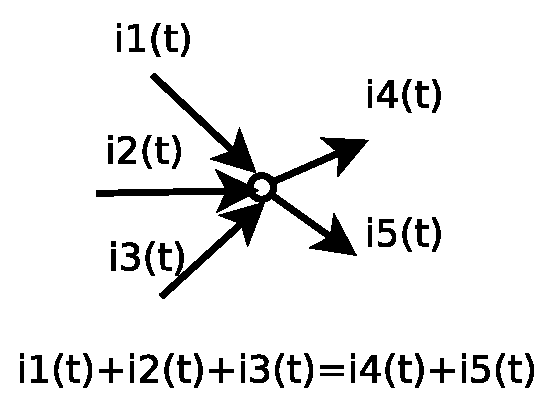
\includegraphics [scale=0.5]{ris1.eps}
    
  \end{figure}
}

  \end{block}
  
\end{frame}

\begin{frame}{Направление электрического тока}
  \begin{block}

    \small{
      Для активного сопротивления - приемника электрической энергии - мощность (скорость преобразования электрической энерии в теплоту) положительна в том и только в том случае, если и падение напряжения, и ток имеют одинаковые знаки, так как $p=ui$.

      Поэтому при постоянных токах для сопротивлений (в общем случае для любых приемников) \textit{положительное направление тока совпадает с положительным направлением напряжения: от плюса к минусу (от более высокого потенциала к более низкому)}.

      В первом законе Кирхгофа токи, направленные от узла, записываются с положительным знаком. Токи, направленные к узлу, записываются со знаком минус. (В тоже время, нужно понимать, что это лишь удобное обозначение. Можно было бы принять и противоположное обозначение).
}

  \end{block}
  
\end{frame}

\begin{frame}{Второй закон Кирхгофа}
  \begin{block}

    \small{
      \textbf{Второй закон Кирхгофа} формулируется для замкнутого контура электрической цепи:
      \textit{В любом замкнутом контуре электрической цепи алгебраическая сумма мнговенных значений ЭДС равна алгебраической сумме мгновенных значений падений напряжения на всех пассивных элементах этого контура: $$\sum_{k=1}^{m}e_k(t)=\sum_{k=1}^{n}u_k(t),$$
        где $m$ - число активных элементов; $n$ - число пассивных элементов.
      }

      Если направление ЭДС или напряжение совпадает с направлением обхода контура, то они суммируются со знаком плюс, а если они противоположны, то суммирование имеет знак минус.

      Для линейных электрических цепей постоянного тока, когда для любого $k$-го сопротивления справедлив закон Ома, второй закон Кирхгофа удобно записывать в виде: $$\sum_{k=1}^{m} E_k=\sum_{k=1}^{n}I_k\cdot R_k$$

      Если ток направлен согласно с направлением обхода контура, слагаемое в правой части берется со знаком плюс, а если противоположно, то со знаком минус.
      
}

  \end{block}
  
\end{frame}

\section{Расчет цепей постоянного тока на основе законов Кирхгофа}
\begin{frame}{Примеры расчета цепей постоянного тока на основе законов Кирхгофа}
  \begin{block}

    \small{
      Любая задача анализа электрической цепи может быть решена на основе первого и второго законов Кирхгофа. Рассмотрим для демонстрации ряд примеров.

      \textbf{Пример 1.} В предложенной схеме определить токи всех ветвей.
      \begin{figure}[htb] 
    \centering
    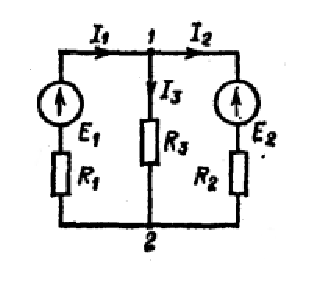
\includegraphics [scale=1.3]{ris2.eps}
  \end{figure}

  В данной схеме выделено два узла $n_{\text{у}}=2$ и имеется три ветви $n_{\text{в}}=3$. Составим уравнение по первому закону Кирхгофа для первого узла: $$I_1=I_2+I_3$$
  Можно также составить аналогичное уравнение и для второго узла: $$I_2+I_3=I_1,$$ но видно, что они ничем друг от друга не отличаются.
}

  \end{block}
  
\end{frame}

\begin{frame}{Пример 1  расчета цепей постоянного тока на основе законов Кирхгофа}
  \begin{block}

    \small{
      Для составления уравнений по второму закону Кирхгофа в схеме нужно выделить замкнутые контура. В предложенной схеме всего можно выделить три таких контура. Направления обхода контуров выбирается произвольно.

      Первый контур:
\begin{figure}[htb] 
    \centering
    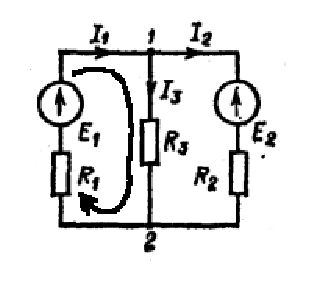
\includegraphics [scale=1.3]{ris3.eps}
  \end{figure}
  Уравнение по второму закону Кирхгофа для этого контура: $$E_1=I_1R_1+I_3R_3$$
      
}

  \end{block}
  
\end{frame}

\begin{frame}{Пример 1  расчета цепей постоянного тока на основе законов Кирхгофа}
  \begin{block}

    \small{
  Второй контур:
\begin{figure}[htb] 
    \centering
    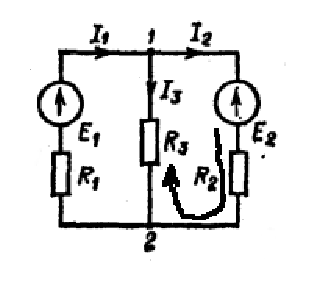
\includegraphics [scale=1.3]{ris4.eps}
  \end{figure}
  Уравнение по второму закону Кирхгофа для этого контура: $$-E_2=I_2R_2-I_3R_3$$
  Следует обратить внимание на знаки: поскольку направление источника напряжения $E_2$ противоположно выбранному направлению, то он берется со знаком минус. Аналогично, ток $I_3$ направлен противоположно выбранному направлению, он тоже берется со знаком минус.
}

  \end{block}
  
\end{frame}

\begin{frame}{Пример 1  расчета цепей постоянного тока на основе законов Кирхгофа}
  \begin{block}

    \small{
  Третий контур:
\begin{figure}[htb] 
    \centering
    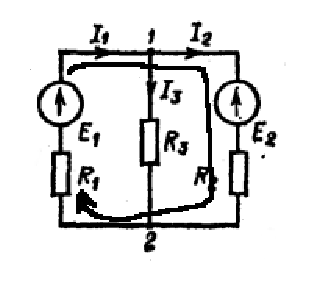
\includegraphics [scale=1.3]{ris5.eps}
  \end{figure}
  Уравнение по второму закону Кирхгофа для этого контура: $$E_1-E_2=I_1R_1+I_2R_2$$
}

  \end{block}
  
\end{frame}

\begin{frame}{Пример 1  расчета цепей постоянного тока на основе законов Кирхгофа}
  \begin{block}

    \small{
      Давайте внимательно посмотрим на полученные уравнения:

      по первому закону Кирхгофа:
      \begin{equation} I_1=I_2+I_3\end{equation}
      \begin{equation}I_2+I_3=I_1\end{equation}
      по второму закону Кирхгофа:
      \begin{equation}E_1=I_1R_1+I_3R_3\end{equation}
      \begin{equation}-E_2=I_2R_2-I_3R_3\end{equation}
      \begin{equation}E_1-E_2=I_1R_1+I_2R_2\end{equation}
      Видно, что из (1) получается (2). Если сложить левые и правые части (3) и (4), то получим (5). Таким образом, полученные уравнения не являются независимыми, и возникает вопрос, сколько уравнений следует оставить, чтобы найти все токи.

      В нашем случае три неизвестных тока требуют три независимых уравнения. Поэтому от первого закона Кирхгофа возьмем, например, уравнение (1), а  от второго закона Кирхгофа возьмем уравнения (3), (4). 
}

  \end{block}
  
\end{frame}

\begin{frame}{Пример 1  расчета цепей постоянного тока на основе законов Кирхгофа}
  \begin{block}

    \small{
      Окончательно, следует решить следующую систему уравнений:
\[
\systeme*{ I_1=I_2+I_3, E_1=I_1R_1+I_3R_3, (-E_2)=I_2R_2-I_3R_3}
\]
Приведя ее к каноническому виду, получим:
\[
\systeme*{I_1-I_2-I_3=0, R_1I_1+0\cdot I_2+R_3I_3=E_1, 0\cdot I_1+R_2I_2-R_3I_3=-E_2}
\]
Последнюю можно решить многими способами, например, методом Крамера:

\begin{equation*} \Delta=\begin{vmatrix} 1 & -1 & -1 \\ R_1 & 0 & R_3 \\ 0 &  R_2 &  -R_3 \end{vmatrix}=-R_1R_2-R_2R_3-R_1R_3\end{equation*}
\begin{equation*} \Delta_{I_1}=\begin{vmatrix} 0 & -1 & -1 \\ E_1 & 0 & R_3 \\ -E_2 &  R_2 &  -R_3 \end{vmatrix}, \Delta_{I_2}=\begin{vmatrix} 1 & 0 & -1 \\ R_1 & E_1 & R_3 \\ 0 &  -E_2 &  -R_3 \end{vmatrix}, \Delta_{I_3}=\begin{vmatrix} 1 & -1 & 0 \\ R_1 & 0 & E_1 \\ 0 &  R_2 &  -E_2 \end{vmatrix}\end{equation*}

}

  \end{block}
  
\end{frame}

\begin{frame}{Пример 1  расчета цепей постоянного тока на основе законов Кирхгофа}
  \begin{block}

    \small{

      $$I_1=\frac{\Delta_{I_1}}{\Delta}, I_2=\frac{\Delta_{I_2}}{\Delta}, I_3=\frac{\Delta_{I_3}}{\Delta}$$
      $$I_1=\frac{-E_1R_2+E_2R_3-E_1R_3}{-R_1R_2-R_2R_3-R_1R_3}, I_2=\frac{-E_1R_3+E_2R_1+E_2R_3}{-R_1R_2-R_2R_3-R_1R_3}, I_3=\frac{-E_1R_2-E_2R_1}{-R_1R_2-R_2R_3-R_1R_3}$$
      На практике выполнять данные преобразования вручную нет необходимости. Целесообразно использовать автоматизированные системы символьных преобразований. Одной из таких систем является система \href{https://ru.wikipedia.org/wiki/Maxima}{Maxima}.
      \begin{figure}[htb] 
    \centering
    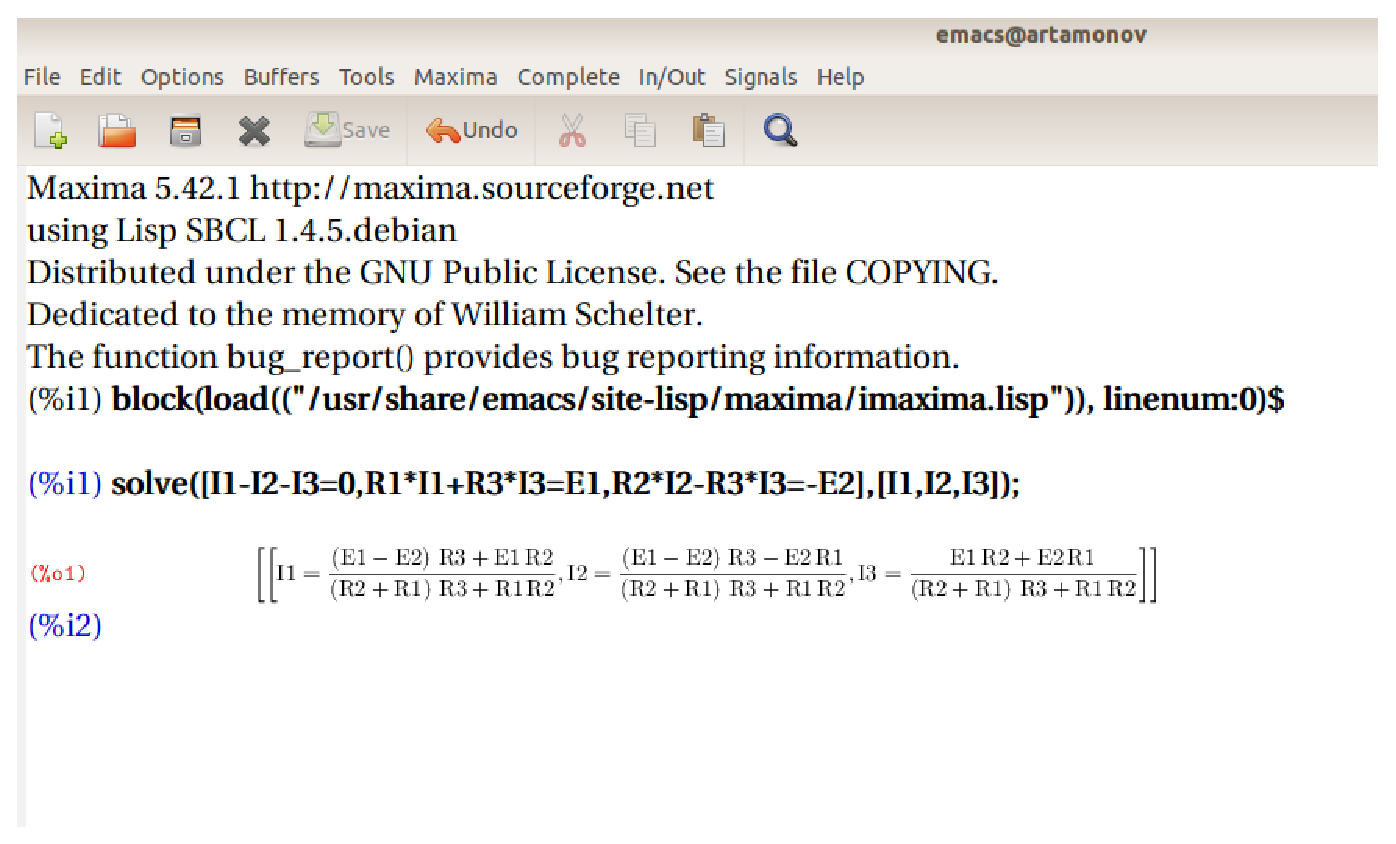
\includegraphics [scale=0.7]{ris6.eps}
  \end{figure}
  Как видно, результаты расчетов совпадают.
}

  \end{block}
  
\end{frame}

\begin{frame}{Пример 1  расчета цепей постоянного тока на основе законов Кирхгофа}
  \begin{block}

    \small{

      Отметим, что чаще всего будет требоваться получить численное значение токов при заданных числовых параметрах. В этом случае можно использовать туже Maxima, но можно использовать и Scilab.

      Зададимся численными значениями параметров схемы и посмотрим, как будут выглядеть расчеты с использованием этих двух сред:
      $$R_1=10 \text{ Ом}, R_2=20 \text{ Ом}, R_3=30 \text{ Ом}, E_1=5 \text{ В}, E_2=3 \text{ В}$$
       \begin{figure}[htb] 
    \centering
    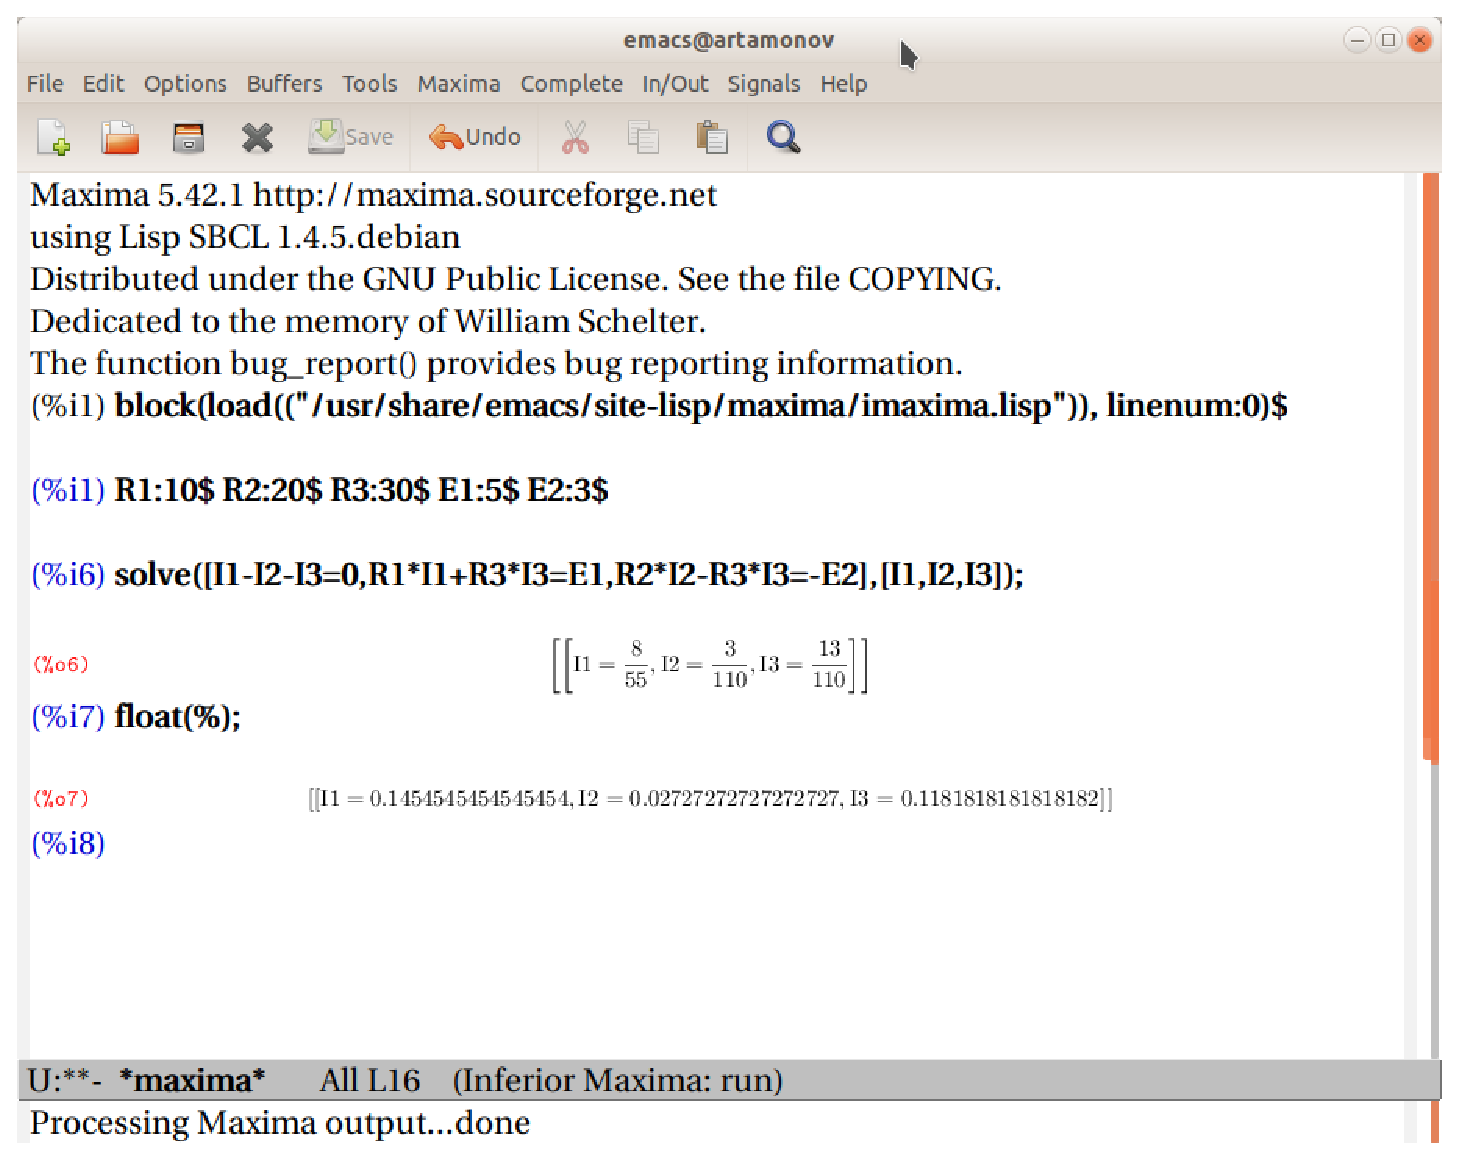
\includegraphics [scale=0.7]{ris7.eps}
  \end{figure}
}

  \end{block}
  
\end{frame}

\begin{frame}{Пример 1  расчета цепей постоянного тока на основе законов Кирхгофа}
  \begin{block}

    \small{

      Для использования Scilab перепишем полученные уравнения в численной форме:
\[
\systeme*{I_1-I_2-I_3=0, 10\cdot I_1+0\cdot I_2+30\cdot I_3=5, 0\cdot I_1+20\cdot I_2-30\cdot I_3=-3}
\]
Тогда имеем:
 \begin{figure}[htb] 
    \centering
    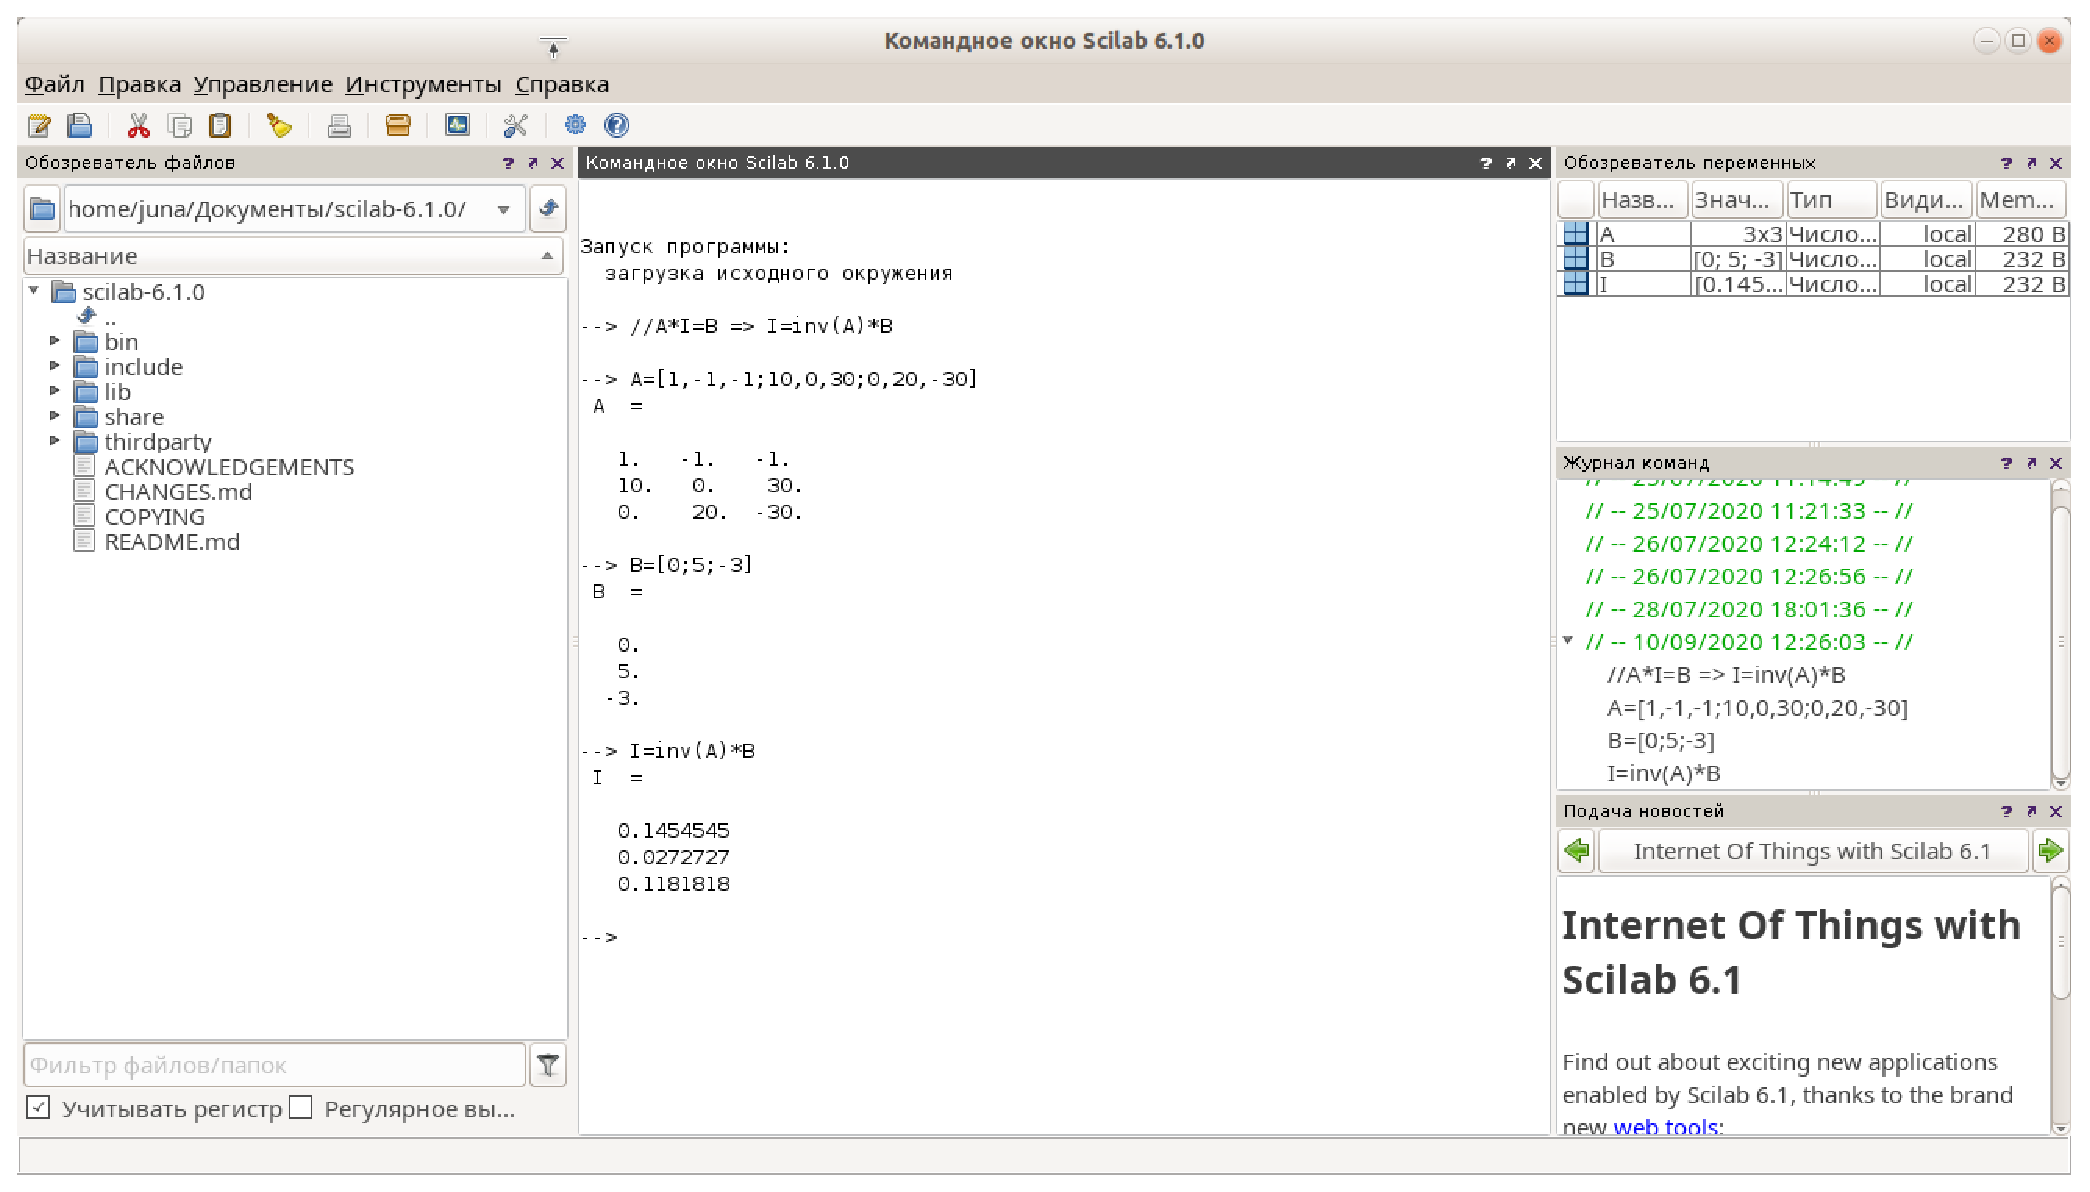
\includegraphics [scale=0.7]{ris8.eps}
  \end{figure}
      

}
  \end{block}
  
\end{frame}

\begin{frame}{Пример 1  расчета цепей постоянного тока на основе законов Кирхгофа}
  \begin{block}

    \small{

 В Scilab можно также смоделировать работу данной схемы в симуляторе xcos.
  \begin{figure}[htb] 
    \centering
    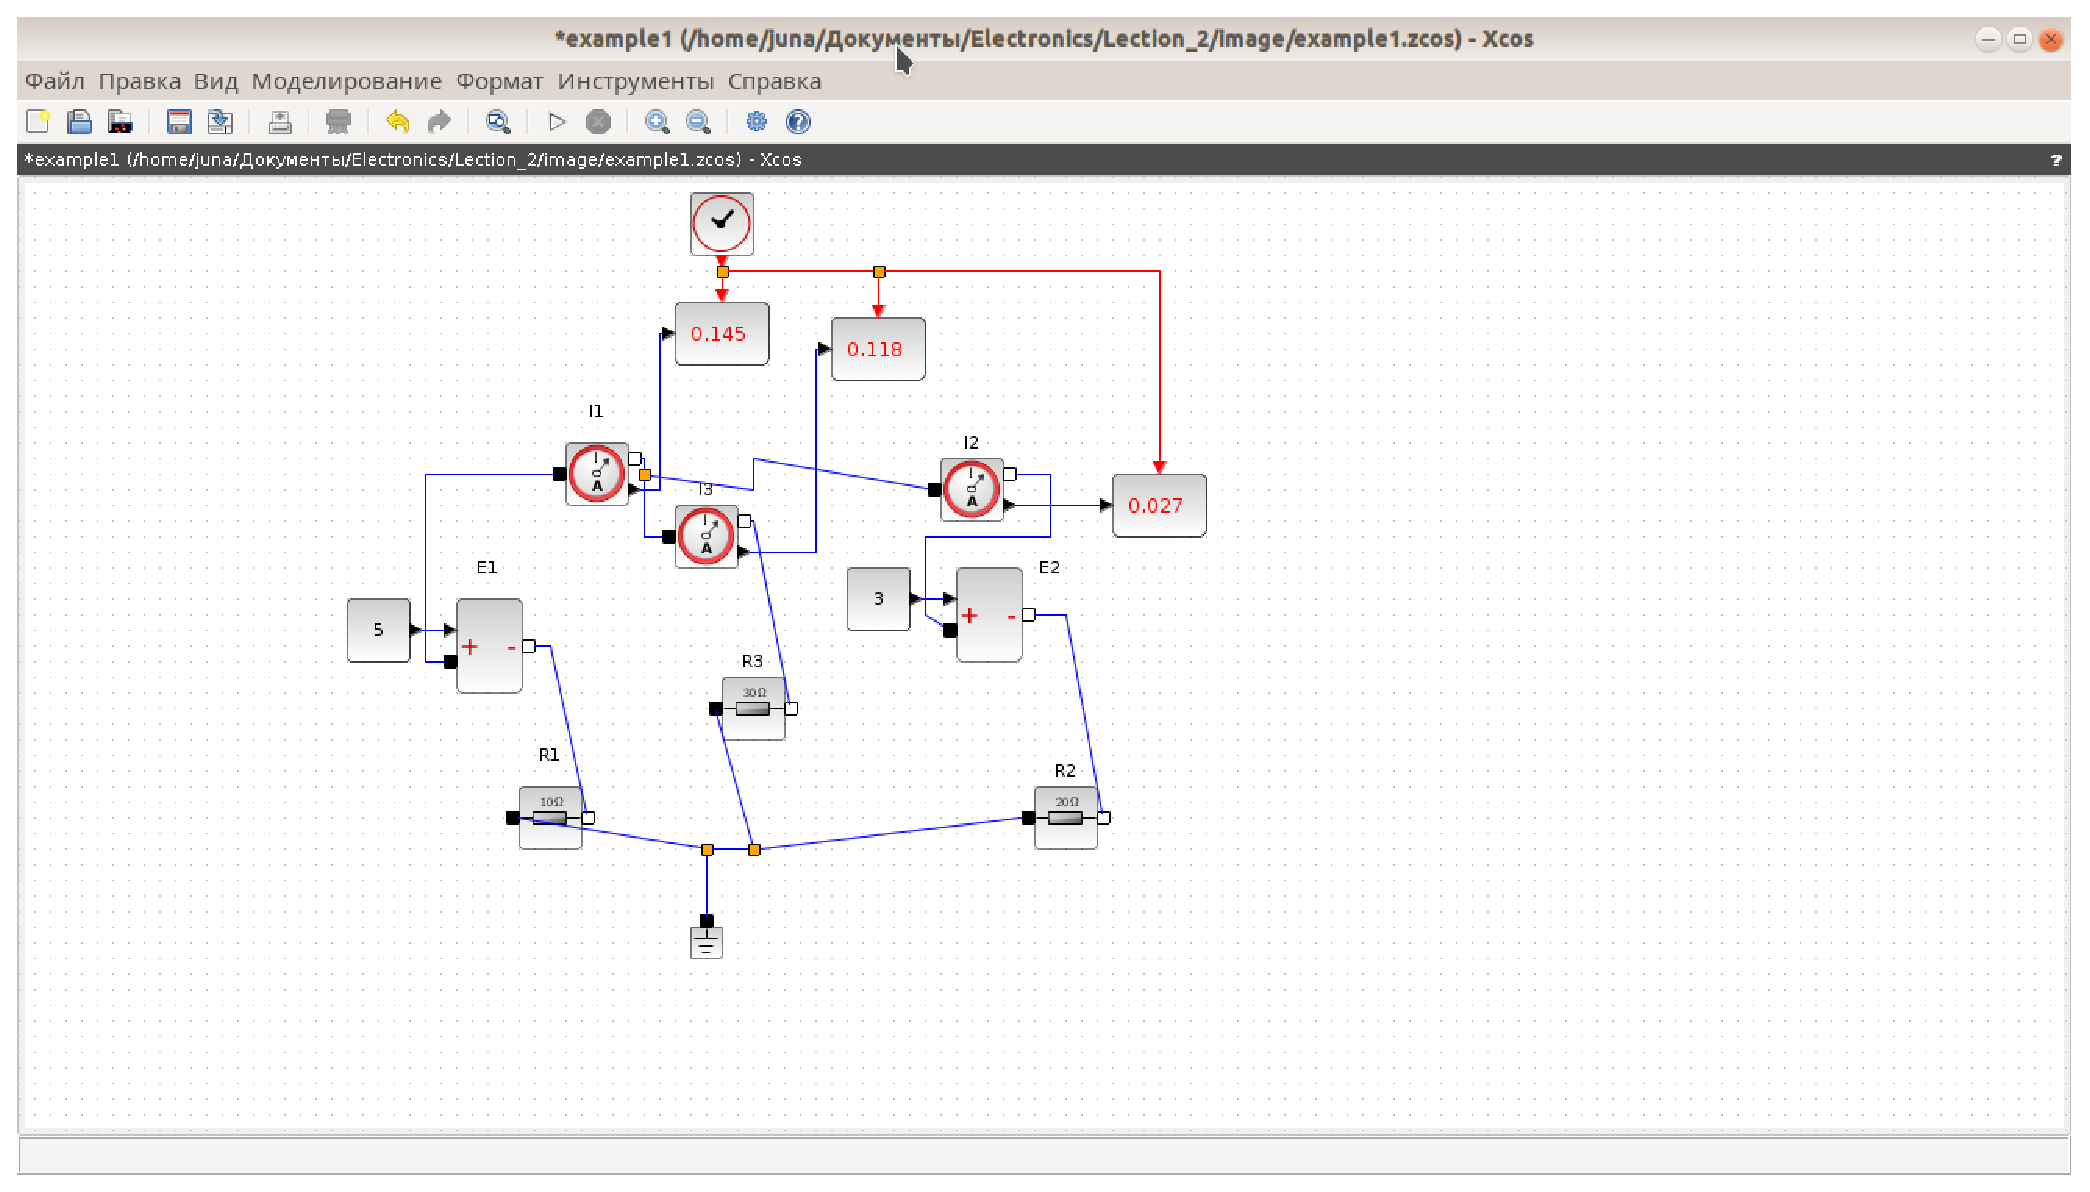
\includegraphics [scale=0.6]{ris9.eps}
  \end{figure}     
Как видно из рисунка, результаты моделирования совпадают с теоретическими расчетами.
}
  \end{block}
  
\end{frame}

\begin{frame}{Количество уравнений при расчета цепей постоянного тока на основе законов Кирхгофа}
  \begin{block}

    \small{

      Как видно из рассмотренного примера, количества уравнений, которые можно составить по законам Кирхгофа избыточно для нахождения всех необходимых неизвестных. Можно задаться вопросом, как определить это количество для общего случая. Будем считать неизвестными - токи в ветвях электрической схемы. Их всегда ровно столько, сколько количество ветвей $n_{\text{в}}$. Тогда количество неизвестных, а значит и количество необходимых уравнений равно количеству ветвей $n_{\text{в}}$.

      Каждая ветвь связывает собой два узла, для одного из которых ток этой ветви является входящим (отрицательным), а для другого узла этот же ток является выходящим (положительным). Поэтому, если составить уравнения по первому закону Кирхгофа для всех узлов $n_{\text{у}}$ схемы, то каждый ток войдет в эти уравнения дважды с разными знаками. Значит сумма всех таких уравнений приведет к тождеству $0=0$. Чтобы убрать эту тавтологию, достаточно убрать одно уравнение.

      Таким образом, \textbf{для нахождения токов всех ветвей схемы по первому закону Кирхгофа необходимо составить $n_{\text{у}}-1$ уравнений.}

      \textbf{Составив таким образом $n_{\text{у}}-1$ уравнений по первому закону Кирхгофа, остается составить еще $n_{\text{в}}-(n_{\text{у}}-1)=n_{\text{в}}-n_{\text{у}}+1$ уравнений по второму закону Кирхгофа.}
}
  \end{block}
  
\end{frame}

\begin{frame}{Пример 2  расчета цепей постоянного тока на основе законов Кирхгофа}
  \begin{block}

    \small{

      Рассмотрим еще примеры расчета цепей на основе законов Кирхгофа, используя полученные результаты.
      \begin{figure}[htb] 
    \centering
    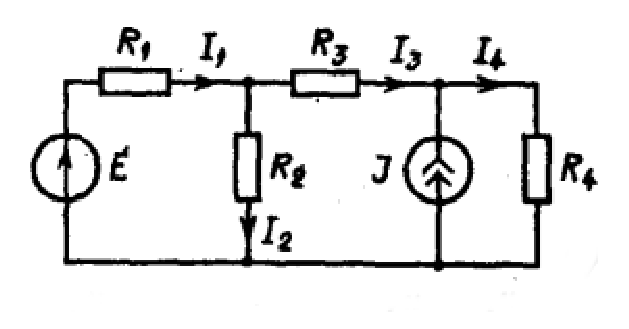
\includegraphics [scale=0.9]{ris10.eps}
  \end{figure}
  Для исходных данных: $E=6 \text{ В}, I=1\text{ А}, R_1=9\text{ Ом}, R_2=4.5\text{ Ом}, R_3=3\text{ Ом}, R_4=6\text{ Ом}$ расчитать все токи ветвей: $I_1, I_2, I_3, I_4$.

  \textit{Решение}. В данной схеме $n_{\text{в}}=5$, $n_{\text{у}}=3$ (заметим, что два узла внизу схемы - это в действительности одно соединение, а значит один узел). Составим два уравнения по первому закону Кирхгофа:
  $$I_1=I_2+I_3$$
  $$I_3+I=I_4$$
  Значит по второму закону Кирхгофа необходимо составить еще $n_{\text{в}}-n_{\text{у}}+1=5-3+1=3$ уравнения.
  
  
}
  \end{block}
  
\end{frame}

\begin{frame}{Пример 2  расчета цепей постоянного тока на основе законов Кирхгофа}
  \begin{block}

    \small{
      Для составления уравнений по второму закону Кирхгофа выберем три произвольных контура.

      Первый контур.
       \begin{figure}[htb] 
    \centering
    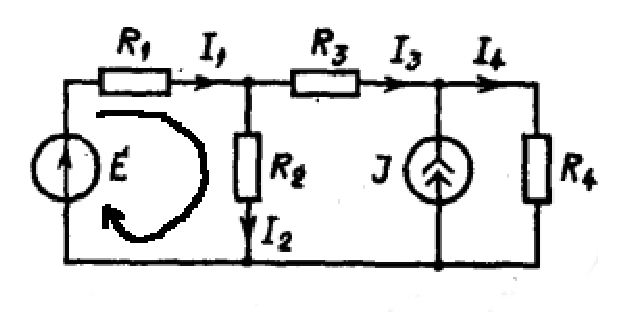
\includegraphics [scale=0.9]{ris11.eps}
  \end{figure}
  $$E=R_1I_1+R_2I_2$$
  Второй контур.
    \begin{figure}[htb] 
    \centering
    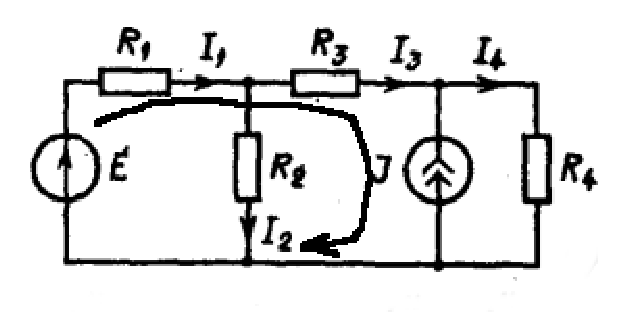
\includegraphics [scale=0.9]{ris12.eps}
  \end{figure}
  $$E=R_1I_1+R_3I_3-U_{I}$$
  
}
  \end{block}
  
\end{frame}

\begin{frame}{Пример 2  расчета цепей постоянного тока на основе законов Кирхгофа}
  \begin{block}

    \small{
      Во втором контуре через $U_{I}$ обозначено напряжение на источнике тока. Поскольку направление источника тока противоположно выбранному направлению обхода, $U_{I}$ в уравнение входит со знаком минус. 

      Обратив внимание на произвольный характер выбора контуров. Например, в качестве альтернативы можно было бы выбрать следующий второй контур:

      Альтернативный второй контур.
      \begin{figure}[htb] 
    \centering
    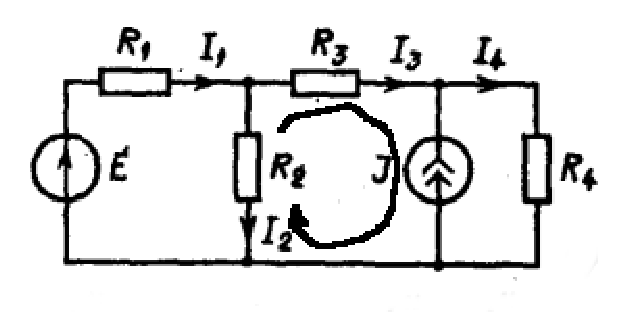
\includegraphics [scale=0.9]{ris13.eps}
  \end{figure}
  $$0=R_3I_3-U_{I}-R_2I_2$$
  Однако важно отметить, что данный контур не может быть выбран как третий независимый. Действительно, если из полученного уравнения $E=R_1I_1+R_3I_3-U_{I}$ вычесть уравнение $E=R_1I_1+R_2I_2$, то как раз получим $0=R_3I_3-U_{I}-R_2I_2$.
}
  \end{block}
  
\end{frame}

\begin{frame}{Пример 2  расчета цепей постоянного тока на основе законов Кирхгофа}
  \begin{block}

    \small{
      Поэтому в качестве третьего контура выберем:
\begin{figure}[htb] 
    \centering
    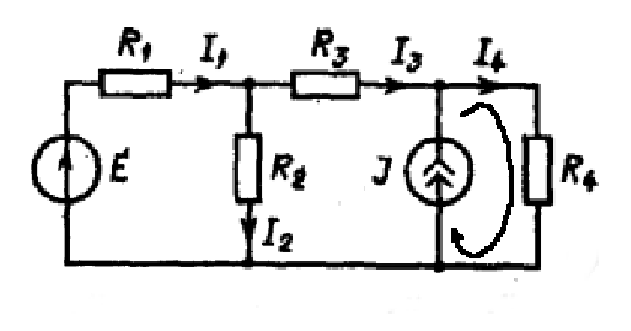
\includegraphics [scale=0.9]{ris14.eps}
  \end{figure}
      $$U_I+R_4I_4=0$$
      Приведем полученные уравнения к канонической форме:
      
      \[
\systeme*{I_1-I_2-I_3+0\cdot I_4+0\cdot U_I=0, 0\cdot I_1+0\cdot I_2-I_3+I_4+0\cdot U_I=I, R_1I_1+R_2I_2+0\cdot I_3+0\cdot I_4+0\cdot U_I=E, 0\cdot I_1-R_2I_2+R_3I_3+0\cdot I_4-U_I=0, 0\cdot I_1+0\cdot I_2+0\cdot I_3+R_4\cdot I_4+U_I=0}
\]
 
}
  \end{block}
  
\end{frame}

\begin{frame}{Пример 2  расчета цепей постоянного тока на основе законов Кирхгофа}
  \begin{block}

    \small{
Подставим числовые значения и проведем расчет в среде Scilab:
  \[
\systeme*{I_1-I_2-I_3+0\cdot I_4+0\cdot U_I=0, 0\cdot I_1+0\cdot I_2-I_3+I_4+0\cdot U_I=1, 9I_1+4.5I_2+0\cdot I_3+0\cdot I_4+0\cdot U_I=6, 0\cdot I_1-4.5I_2+3I_3+0\cdot I_4-U_I=0, 0\cdot I_1+0\cdot I_2+0\cdot I_3+6\cdot I_4+U_I=0}
\]
}
  \end{block}
  
\end{frame}

\begin{frame}{Пример 2  расчета цепей постоянного тока на основе законов Кирхгофа}
  \begin{block}

    \small{

  \begin{figure}[htb] 
    \centering
    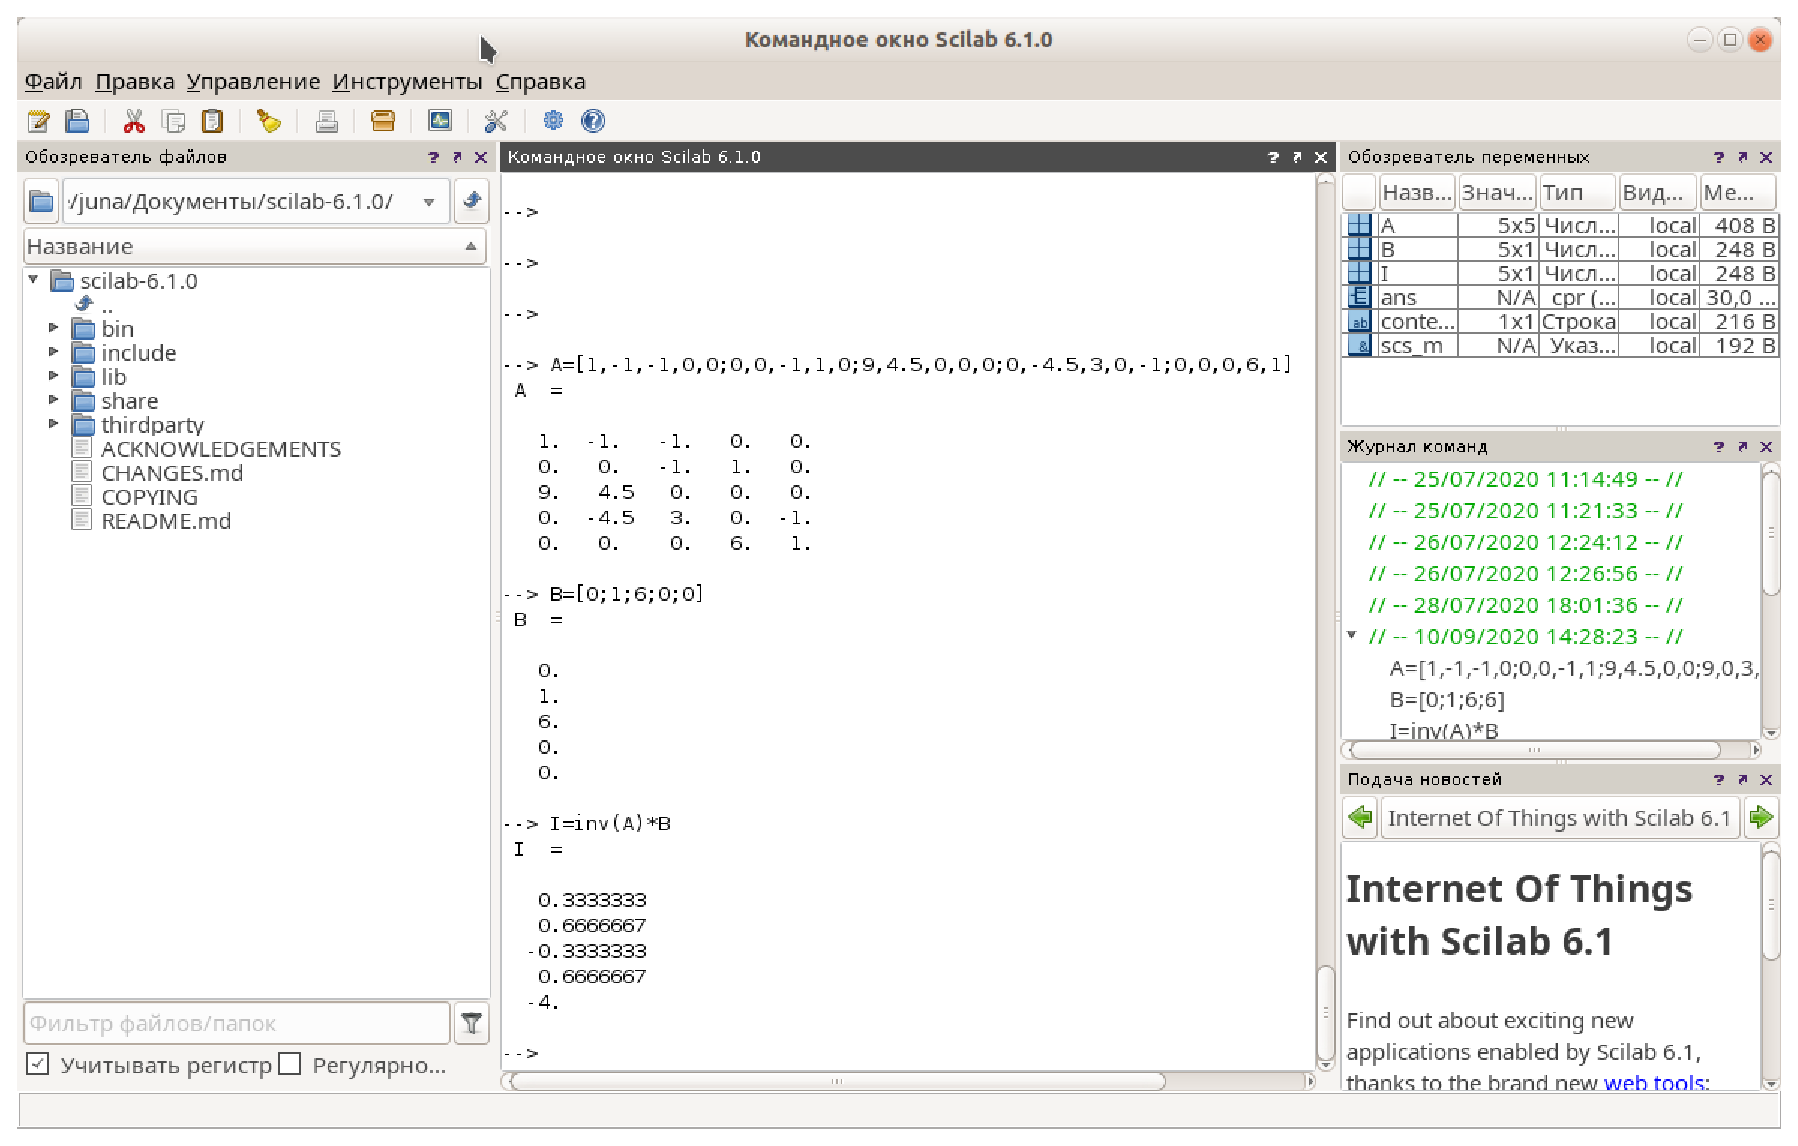
\includegraphics [scale=0.6]{ris15.eps}
  \end{figure}
  Обратите внимание, последнее значение $-4$ - это напряжение на источнике тока. Ток $I_4$ можно выразить по закону Ома $U_I=I_4R_4\Rightarrow I_4=\frac{U_I}{R_4}=\frac{-4}{6}=-0.67 A$. Отрицательное значение говорит о несовпадении выбранного направления тока с действительным направлением в схеме.
}
  \end{block}
  
\end{frame}

\begin{frame}{Пример 3 расчета цепей постоянного тока на основе законов Кирхгофа}
  \begin{block}

    \small{
Рассмотрим еще один важный с точки зрения приложений пример - мостовая схема.
\begin{figure}[htb] 
    \centering
    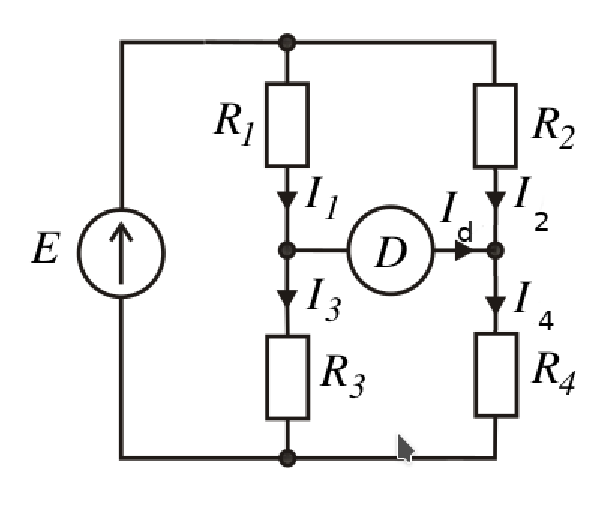
\includegraphics [scale=0.9]{ris16.eps}
  \end{figure}
  Выяснить условия, при которых индикатор $D$ (внутреннее сопротивление близко к нулю) показывает ток $I_D=0 A$.
}
  \end{block}
  
\end{frame}

\begin{frame}{Пример 3 расчета цепей постоянного тока на основе законов Кирхгофа}
  \begin{block}

    \small{
      Составим уравнения по законам Кирхгофа:
    \[
\systeme*{I_1=I_d+I_3, I_4=I_d+I_2,E=I_2R_2+I_4R_4, E=I_1R_1+I_3R_3, 0=I_2R_2-I_1R_1}
\]
Для нахождения символьного результата очень удобно использовать среду Maxima.
}
  \end{block}
  
\end{frame}

\begin{frame}{Пример 3 расчета цепей постоянного тока на основе законов Кирхгофа}
  \begin{block}

    \small{
\begin{figure}[htb] 
    \centering
    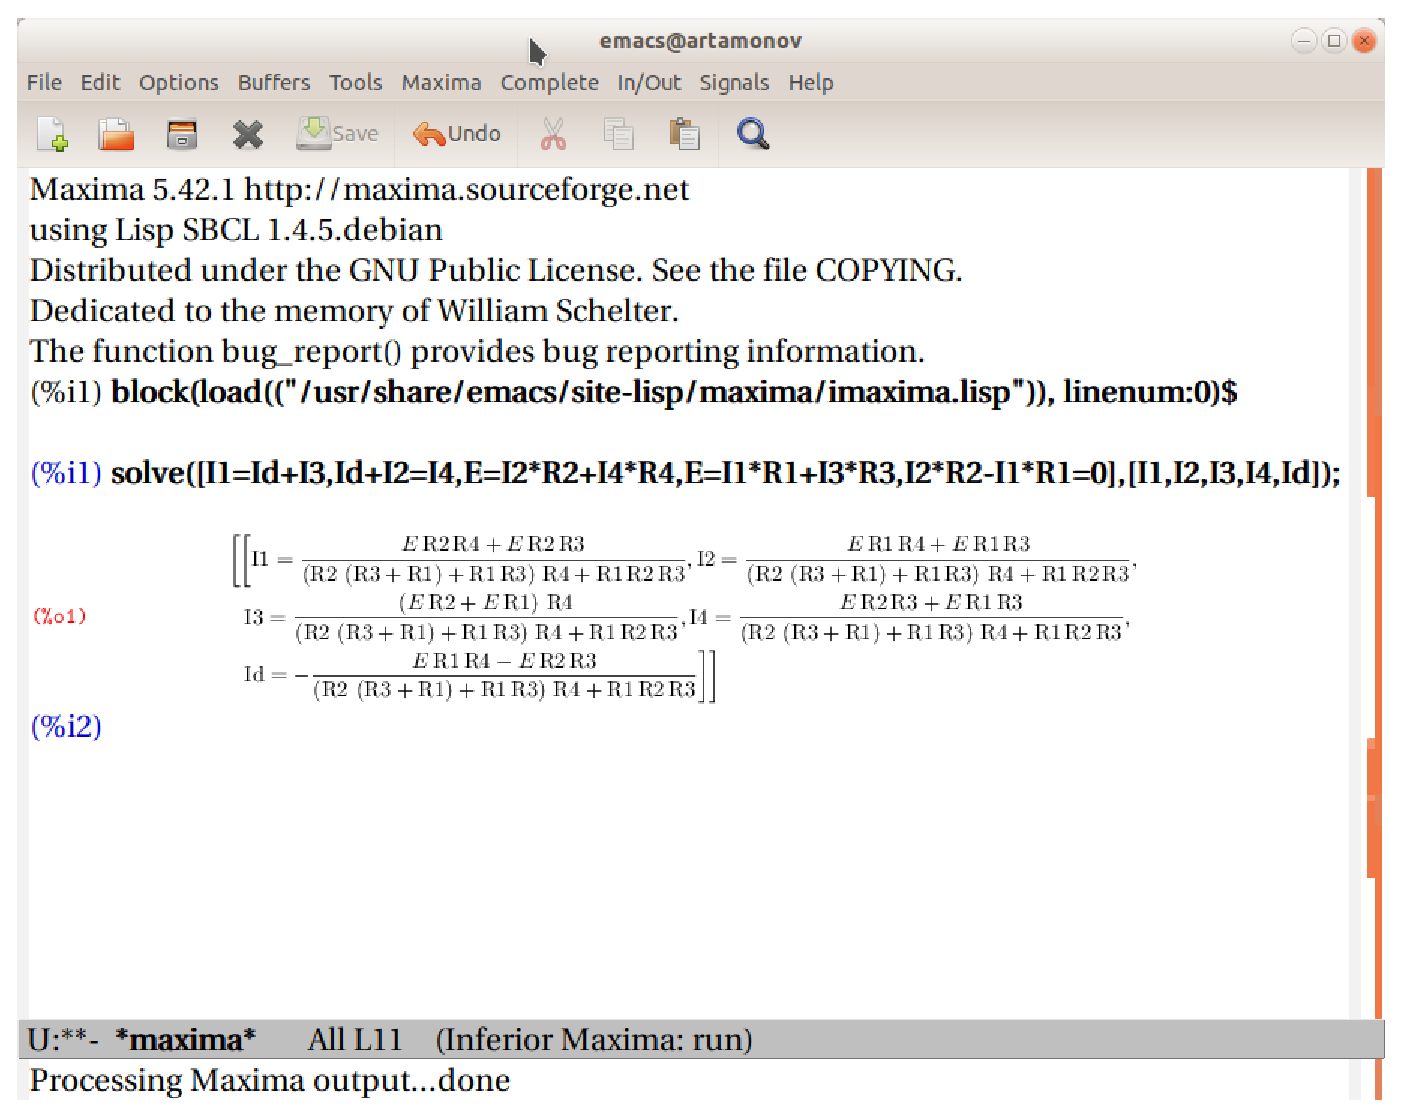
\includegraphics [scale=0.8]{ris17.eps}
  \end{figure}
}
  \end{block}
  
\end{frame}

\begin{frame}{Пример 3 расчета цепей постоянного тока на основе законов Кирхгофа}
  \begin{block}

    \small{
Из полученного результата видно, что необходимым условием $I_d=0$ является соотношение $R_1R_4-R_2R_3=0$. Это условие и называется условием равновесия моста. Данная схема носит название моста Уитстона и используется для измерения сопротивлений. Если $R_4$ - неизвестное сопротивление, а $R_1,R_2,R_3$ - регулировочные сопротивления, то для определения $R_4$ необходимо регулировать $R_1,R_2,R_3$ до тех пор, пока ток через индикатор $D$ не станет равен нулю. Тогда неизвестное сопротивление определяется из соотношения: $$R_4=\frac{R_2R_3}{R_1}$$
}
  \end{block}
  
\end{frame}

\section{Расчет цепей постоянного тока на основе метода контурных токов}
\begin{frame}{Метод контурных токов}
  \begin{block}

    \small{
      При расчете сложной электрической цепи с использованием законов Кирхгофа решения получаются громозкими из-за большого числа уравнений. Это количество можно сократить, если ввести в расмотрение так называемые контурные токи, обтекающие выбранные независимые контуры. Рассмотрим этот метод на примере следующего рисунка.
      \begin{figure}[htb] 
    \centering
    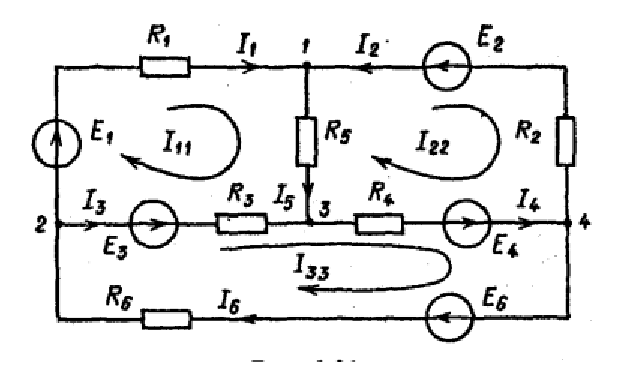
\includegraphics [scale=1.0]{ris18.eps}
  \end{figure}
}
Контурный ток является одинаковым для всех ветвей рассматриваемого контура. Чтобы отличать контурные токи от токов ветвей, часто их индексация проводится двойными цифрами, как показано на рисунке. Из рисунка имеем следующие соотношения между контурными токами и токами ветвей:
$$I_1=I_{11}, I_2=-I_{22}, I_6=I_{33}$$
  \end{block}
  
\end{frame}

\begin{frame}{Метод контурных токов}
  \begin{block}

    \small{
      Токи внутренних ветвей, относящиеся к двум смежным контурам, находим как алгебраическую сумму контурных токов, протекающих по этим ветвям:
      $$I_5=I_{11}-I_{22}, I_3=I_{33}-I_{11}, I_4=I_{33}-I_{22}.$$

      Теперь остается вместо шести величин найти три величины - контурные токи $I_{11},I_{22},I_{33}$. Для этого вводится ряд дополнительных понятий.

      \textbf{Контурной ЭДС} называют алгебраическую сумму всех ЭДС данного контура:
      $$E_{11}=E_1-E_3, E_{22}=-E_2-E_4, E_{33}=E_3+E_4+E_6$$
      Сумма сопротивлений ветвей, образующих контур, называется \textbf{собственным сопротивлением контура}. Собственные сопротивления контуров также обозначаются двойными одинаковыми индексами:
      $$R_{11}=R_1+R_3+R_5, R_{22}=R_2+R_4+R_5, R_{33}=R_3+R_4+R_6$$
      Сопротивление ветви, принадлежащей двум смежным контурам, называют \textbf{общим сопротивлением контуров}. Их обозначают двойными индексами по номерам смежных контуров. В нашем примере сопротивление $R_5$ расположено на границе первого и второго контуров $R_{12}=R_{21}=R_5$.
      }
  \end{block}
  
\end{frame}

\begin{frame}{Метод контурных токов}
  \begin{block}

    \small{
      Используя введенные понятия, составляется система контурных уравнений. Каждое контурное уравнение составляется по правилу: \textbf{контурная ЭДС равна сумме падений напряжения на собственных и общих сопротивлениях контуров при протекании контурных токов.}
      Используя это правило, составим три уравнения в нашей задаче:
      $$E_{11}=R_{11}I_{11}-R_{12}I_{22}-R_{13}I_{33}$$
      $$E_{22}=-R_{21}I_{11}+R_{22}I_{22}-R_{23}I_{33}$$
      $$E_{33}=-R_{31}I_{11}-R_{32}I_{22}+R_{33}I_{33}$$
      }
  \end{block}
  
\end{frame}

\begin{frame}{Пример использования метода контурных токов}
  \begin{block}

    \small{
      Рассмотрим задачу из примера 1:
\begin{figure}[htb] 
    \centering
    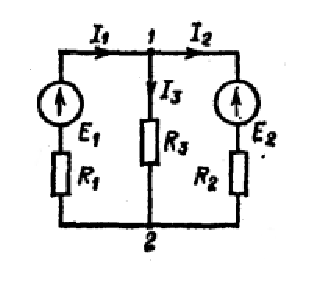
\includegraphics [scale=1.3]{ris2.eps}
  \end{figure}
   $$R_1=10 \text{ Ом}, R_2=20 \text{ Ом}, R_3=30 \text{ Ом}, E_1=5 \text{ В}, E_2=3 \text{ В}$$   
      }
  \end{block}
  
\end{frame}

\begin{frame}{Пример использования метода контурных токов}
  \begin{block}

    \small{
      На следующем рисунке введены контурные токи
\begin{figure}[htb] 
    \centering
    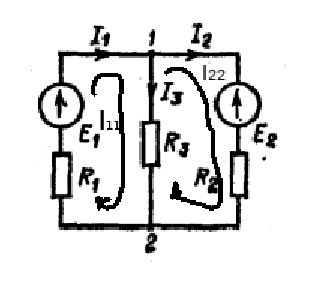
\includegraphics [scale=1.3]{ris19.eps}
  \end{figure}
  Имеем: $$E_{11}=E_1=5, E_{22}=-E_2=-3$$
  $$R_{11}=R_1+R_3=40, R_{22}=R_2+R_3=50, R_{12}=R_{21}=R_3=30$$
  $$I_1=I_{11}, I_2=I_{22},I_3=I_{11}-I_{22}$$
  Составим систему уравнений по методу контурных токов:
  $$E_{11}=R_{11}I_{11}-R_{12}I_{22}$$
  $$E_{22}=-R_{21}I_{11}+R_{22}I_{22}$$
  Подставляя численные значения, имеем: $5=40I_{11}-30I_{22}, -3=-30I_{11}+50I_{22}$. Теперь уже легко найти $I_{11}=I_1=\frac{8}{55}\approx 0.145, I_{22}=I_2=\frac{3}{110}\approx 0.027, I_3=\frac{8}{55}-\frac{3}{110}=\frac{13}{110}\approx 0.118$
      }
  \end{block}
  
\end{frame}

\begin{comment}
\section{Эквивалентные преобразования электрических цепей при последовательном, параллельном и смешанном соединении сопротивлений}
\begin{frame}{Первый закон Кирхгофа}
  \begin{block}

    \small{
   
}

  \end{block}
  
\end{frame}

\section{Преобразование треугольника сопротивлений в здезду и обратное преобразование}

\begin{frame}{Первый закон Кирхгофа}
  \begin{block}

    \small{
   
}

  \end{block}
  
\end{frame}

\section{Преобразование схем источников напряжения и тока}

\begin{frame}{Первый закон Кирхгофа}
  \begin{block}

    \small{
   
}

  \end{block}
  
\end{frame}
\end{comment}

\end{document}
